\documentclass{article}
% Configuration for the memoir class.
\renewcommand{\cleardoublepage}{}
% \renewcommand*{\partpageend}{}
\renewcommand{\afterpartskip}{}
\maxsecnumdepth{subsubsection} % number subsections
\maxtocdepth{subsubsection}

\addtolength{\parindent}{-5mm}
% Packages not included:
% For multiline comments, use caption package. But this conflicts with hyperref while making html files.
% subfigure conflicts with use with memoir style-sheet.

% Use something like:
% % Use something like:
% % Use something like:
% \input{../../macros}

% groupings of objects.
\newcommand{\set}[1]{\left\{ #1 \right\}}
\newcommand{\seq}[1]{\left(#1\right)}
\newcommand{\ang}[1]{\langle#1\rangle}
\newcommand{\tuple}[1]{\left(#1\right)}

% numerical shortcuts.
\newcommand{\abs}[1]{\left| #1\right|}
\newcommand{\floor}[1]{\left\lfloor #1 \right\rfloor}
\newcommand{\ceil}[1]{\left\lceil #1 \right\rceil}

% linear algebra shortcuts.
\newcommand{\change}{\Delta}
\newcommand{\norm}[1]{\left\| #1\right\|}
\newcommand{\dprod}[1]{\langle#1\rangle}
\newcommand{\linspan}[1]{\langle#1\rangle}
\newcommand{\conj}[1]{\overline{#1}}
\newcommand{\gradient}{\nabla}
\newcommand{\der}{\frac{d}{dx}}
\newcommand{\lap}{\Delta}
\newcommand{\kron}{\otimes}
\newcommand{\nperp}{\nvdash}

\newcommand{\mat}[1]{\left( \begin{smallmatrix}#1 \end{smallmatrix} \right)}

% derivatives and limits
\newcommand{\partder}[2]{\frac{\partial #1}{\partial #2}}
\newcommand{\partdern}[3]{\frac{\partial^{#3} #1}{\partial #2^{#3}}}

% Arrows
\newcommand{\diverge}{\nearrow}
\newcommand{\notto}{\nrightarrow}
\newcommand{\up}{\uparrow}
\newcommand{\down}{\downarrow}
% gets and gives are defined!

% ordering operators
\newcommand{\oleq}{\preceq}
\newcommand{\ogeq}{\succeq}

% programming and logic operators
\newcommand{\dfn}{:=}
\newcommand{\assign}{:=}
\newcommand{\co}{\ co\ }
\newcommand{\en}{\ en\ }


% logic operators
\newcommand{\xor}{\oplus}
\newcommand{\Land}{\bigwedge}
\newcommand{\Lor}{\bigvee}
\newcommand{\finish}{$\Box$}
\newcommand{\contra}{\Rightarrow \Leftarrow}
\newcommand{\iseq}{\stackrel{_?}{=}}


% Set theory
\newcommand{\symdiff}{\Delta}
\newcommand{\union}{\cup}
\newcommand{\inters}{\cap}
\newcommand{\Union}{\bigcup}
\newcommand{\Inters}{\bigcap}
\newcommand{\nullSet}{\phi}

% graph theory
\newcommand{\nbd}{\Gamma}

% Script alphabets
% For reals, use \Re

% greek letters
\newcommand{\eps}{\epsilon}
\newcommand{\del}{\delta}
\newcommand{\ga}{\alpha}
\newcommand{\gb}{\beta}
\newcommand{\gd}{\del}
\newcommand{\gf}{\phi}
\newcommand{\gF}{\Phi}
\newcommand{\gl}{\lambda}
\newcommand{\gm}{\mu}
\newcommand{\gn}{\nu}
\newcommand{\gr}{\rho}
\newcommand{\gs}{\sigma}
\newcommand{\gt}{\theta}
\newcommand{\gx}{\xi}

\newcommand{\sw}{\sigma}
\newcommand{\SW}{\Sigma}
\newcommand{\ew}{\lambda}
\newcommand{\EW}{\Lambda}

\newcommand{\Del}{\Delta}
\newcommand{\gD}{\Delta}
\newcommand{\gG}{\Gamma}
\newcommand{\gO}{\Omega}
\newcommand{\gL}{\Lambda}
\newcommand{\gS}{\Sigma}

% Formatting shortcuts
\newcommand{\red}[1]{\textcolor{red}{#1}}
\newcommand{\blue}[1]{\textcolor{blue}{#1}}
\newcommand{\htext}[2]{\texorpdfstring{#1}{#2}}

% Statistics
\newcommand{\distr}{\sim}
\newcommand{\stddev}{\sigma}
\newcommand{\covmatrix}{\Sigma}
\newcommand{\mean}{\mu}
\newcommand{\param}{\gt}
\newcommand{\ftr}{\phi}

% General utility
\newcommand{\todo}[1]{\footnote{TODO: #1}}
\newcommand{\exclaim}[1]{{\textbf{\textit{#1}}}}
\newcommand{\tbc}{[\textbf{Incomplete}]}
\newcommand{\chk}{[\textbf{Check}]}
\newcommand{\oprob}{[\textbf{OP}]:}
\newcommand{\core}[1]{\textbf{Core Idea:}}
\newcommand{\why}{[\textbf{Find proof}]}
\newcommand{\opt}[1]{\textit{#1}}


\DeclareMathOperator*{\argmin}{arg\,min}
\DeclareMathOperator{\rank}{rank}
\newcommand{\redcol}[1]{\textcolor{red}{#1}}
\newcommand{\bluecol}[1]{\textcolor{blue}{#1}}
\newcommand{\greencol}[1]{\textcolor{green}{#1}}


\renewcommand{\~}{\htext{$\sim$}{~}}


% groupings of objects.
\newcommand{\set}[1]{\left\{ #1 \right\}}
\newcommand{\seq}[1]{\left(#1\right)}
\newcommand{\ang}[1]{\langle#1\rangle}
\newcommand{\tuple}[1]{\left(#1\right)}

% numerical shortcuts.
\newcommand{\abs}[1]{\left| #1\right|}
\newcommand{\floor}[1]{\left\lfloor #1 \right\rfloor}
\newcommand{\ceil}[1]{\left\lceil #1 \right\rceil}

% linear algebra shortcuts.
\newcommand{\change}{\Delta}
\newcommand{\norm}[1]{\left\| #1\right\|}
\newcommand{\dprod}[1]{\langle#1\rangle}
\newcommand{\linspan}[1]{\langle#1\rangle}
\newcommand{\conj}[1]{\overline{#1}}
\newcommand{\gradient}{\nabla}
\newcommand{\der}{\frac{d}{dx}}
\newcommand{\lap}{\Delta}
\newcommand{\kron}{\otimes}
\newcommand{\nperp}{\nvdash}

\newcommand{\mat}[1]{\left( \begin{smallmatrix}#1 \end{smallmatrix} \right)}

% derivatives and limits
\newcommand{\partder}[2]{\frac{\partial #1}{\partial #2}}
\newcommand{\partdern}[3]{\frac{\partial^{#3} #1}{\partial #2^{#3}}}

% Arrows
\newcommand{\diverge}{\nearrow}
\newcommand{\notto}{\nrightarrow}
\newcommand{\up}{\uparrow}
\newcommand{\down}{\downarrow}
% gets and gives are defined!

% ordering operators
\newcommand{\oleq}{\preceq}
\newcommand{\ogeq}{\succeq}

% programming and logic operators
\newcommand{\dfn}{:=}
\newcommand{\assign}{:=}
\newcommand{\co}{\ co\ }
\newcommand{\en}{\ en\ }


% logic operators
\newcommand{\xor}{\oplus}
\newcommand{\Land}{\bigwedge}
\newcommand{\Lor}{\bigvee}
\newcommand{\finish}{$\Box$}
\newcommand{\contra}{\Rightarrow \Leftarrow}
\newcommand{\iseq}{\stackrel{_?}{=}}


% Set theory
\newcommand{\symdiff}{\Delta}
\newcommand{\union}{\cup}
\newcommand{\inters}{\cap}
\newcommand{\Union}{\bigcup}
\newcommand{\Inters}{\bigcap}
\newcommand{\nullSet}{\phi}

% graph theory
\newcommand{\nbd}{\Gamma}

% Script alphabets
% For reals, use \Re

% greek letters
\newcommand{\eps}{\epsilon}
\newcommand{\del}{\delta}
\newcommand{\ga}{\alpha}
\newcommand{\gb}{\beta}
\newcommand{\gd}{\del}
\newcommand{\gf}{\phi}
\newcommand{\gF}{\Phi}
\newcommand{\gl}{\lambda}
\newcommand{\gm}{\mu}
\newcommand{\gn}{\nu}
\newcommand{\gr}{\rho}
\newcommand{\gs}{\sigma}
\newcommand{\gt}{\theta}
\newcommand{\gx}{\xi}

\newcommand{\sw}{\sigma}
\newcommand{\SW}{\Sigma}
\newcommand{\ew}{\lambda}
\newcommand{\EW}{\Lambda}

\newcommand{\Del}{\Delta}
\newcommand{\gD}{\Delta}
\newcommand{\gG}{\Gamma}
\newcommand{\gO}{\Omega}
\newcommand{\gL}{\Lambda}
\newcommand{\gS}{\Sigma}

% Formatting shortcuts
\newcommand{\red}[1]{\textcolor{red}{#1}}
\newcommand{\blue}[1]{\textcolor{blue}{#1}}
\newcommand{\htext}[2]{\texorpdfstring{#1}{#2}}

% Statistics
\newcommand{\distr}{\sim}
\newcommand{\stddev}{\sigma}
\newcommand{\covmatrix}{\Sigma}
\newcommand{\mean}{\mu}
\newcommand{\param}{\gt}
\newcommand{\ftr}{\phi}

% General utility
\newcommand{\todo}[1]{\footnote{TODO: #1}}
\newcommand{\exclaim}[1]{{\textbf{\textit{#1}}}}
\newcommand{\tbc}{[\textbf{Incomplete}]}
\newcommand{\chk}{[\textbf{Check}]}
\newcommand{\oprob}{[\textbf{OP}]:}
\newcommand{\core}[1]{\textbf{Core Idea:}}
\newcommand{\why}{[\textbf{Find proof}]}
\newcommand{\opt}[1]{\textit{#1}}


\DeclareMathOperator*{\argmin}{arg\,min}
\DeclareMathOperator{\rank}{rank}
\newcommand{\redcol}[1]{\textcolor{red}{#1}}
\newcommand{\bluecol}[1]{\textcolor{blue}{#1}}
\newcommand{\greencol}[1]{\textcolor{green}{#1}}


\renewcommand{\~}{\htext{$\sim$}{~}}


% groupings of objects.
\newcommand{\set}[1]{\left\{ #1 \right\}}
\newcommand{\seq}[1]{\left(#1\right)}
\newcommand{\ang}[1]{\langle#1\rangle}
\newcommand{\tuple}[1]{\left(#1\right)}

% numerical shortcuts.
\newcommand{\abs}[1]{\left| #1\right|}
\newcommand{\floor}[1]{\left\lfloor #1 \right\rfloor}
\newcommand{\ceil}[1]{\left\lceil #1 \right\rceil}

% linear algebra shortcuts.
\newcommand{\change}{\Delta}
\newcommand{\norm}[1]{\left\| #1\right\|}
\newcommand{\dprod}[1]{\langle#1\rangle}
\newcommand{\linspan}[1]{\langle#1\rangle}
\newcommand{\conj}[1]{\overline{#1}}
\newcommand{\gradient}{\nabla}
\newcommand{\der}{\frac{d}{dx}}
\newcommand{\lap}{\Delta}
\newcommand{\kron}{\otimes}
\newcommand{\nperp}{\nvdash}

\newcommand{\mat}[1]{\left( \begin{smallmatrix}#1 \end{smallmatrix} \right)}

% derivatives and limits
\newcommand{\partder}[2]{\frac{\partial #1}{\partial #2}}
\newcommand{\partdern}[3]{\frac{\partial^{#3} #1}{\partial #2^{#3}}}

% Arrows
\newcommand{\diverge}{\nearrow}
\newcommand{\notto}{\nrightarrow}
\newcommand{\up}{\uparrow}
\newcommand{\down}{\downarrow}
% gets and gives are defined!

% ordering operators
\newcommand{\oleq}{\preceq}
\newcommand{\ogeq}{\succeq}

% programming and logic operators
\newcommand{\dfn}{:=}
\newcommand{\assign}{:=}
\newcommand{\co}{\ co\ }
\newcommand{\en}{\ en\ }


% logic operators
\newcommand{\xor}{\oplus}
\newcommand{\Land}{\bigwedge}
\newcommand{\Lor}{\bigvee}
\newcommand{\finish}{$\Box$}
\newcommand{\contra}{\Rightarrow \Leftarrow}
\newcommand{\iseq}{\stackrel{_?}{=}}


% Set theory
\newcommand{\symdiff}{\Delta}
\newcommand{\union}{\cup}
\newcommand{\inters}{\cap}
\newcommand{\Union}{\bigcup}
\newcommand{\Inters}{\bigcap}
\newcommand{\nullSet}{\phi}

% graph theory
\newcommand{\nbd}{\Gamma}

% Script alphabets
% For reals, use \Re

% greek letters
\newcommand{\eps}{\epsilon}
\newcommand{\del}{\delta}
\newcommand{\ga}{\alpha}
\newcommand{\gb}{\beta}
\newcommand{\gd}{\del}
\newcommand{\gf}{\phi}
\newcommand{\gF}{\Phi}
\newcommand{\gl}{\lambda}
\newcommand{\gm}{\mu}
\newcommand{\gn}{\nu}
\newcommand{\gr}{\rho}
\newcommand{\gs}{\sigma}
\newcommand{\gt}{\theta}
\newcommand{\gx}{\xi}

\newcommand{\sw}{\sigma}
\newcommand{\SW}{\Sigma}
\newcommand{\ew}{\lambda}
\newcommand{\EW}{\Lambda}

\newcommand{\Del}{\Delta}
\newcommand{\gD}{\Delta}
\newcommand{\gG}{\Gamma}
\newcommand{\gO}{\Omega}
\newcommand{\gL}{\Lambda}
\newcommand{\gS}{\Sigma}

% Formatting shortcuts
\newcommand{\red}[1]{\textcolor{red}{#1}}
\newcommand{\blue}[1]{\textcolor{blue}{#1}}
\newcommand{\htext}[2]{\texorpdfstring{#1}{#2}}

% Statistics
\newcommand{\distr}{\sim}
\newcommand{\stddev}{\sigma}
\newcommand{\covmatrix}{\Sigma}
\newcommand{\mean}{\mu}
\newcommand{\param}{\gt}
\newcommand{\ftr}{\phi}

% General utility
\newcommand{\todo}[1]{\footnote{TODO: #1}}
\newcommand{\exclaim}[1]{{\textbf{\textit{#1}}}}
\newcommand{\tbc}{[\textbf{Incomplete}]}
\newcommand{\chk}{[\textbf{Check}]}
\newcommand{\oprob}{[\textbf{OP}]:}
\newcommand{\core}[1]{\textbf{Core Idea:}}
\newcommand{\why}{[\textbf{Find proof}]}
\newcommand{\opt}[1]{\textit{#1}}


\DeclareMathOperator*{\argmin}{arg\,min}
\DeclareMathOperator{\rank}{rank}
\newcommand{\redcol}[1]{\textcolor{red}{#1}}
\newcommand{\bluecol}[1]{\textcolor{blue}{#1}}
\newcommand{\greencol}[1]{\textcolor{green}{#1}}


\renewcommand{\~}{\htext{$\sim$}{~}}



%opening
\title{Data mining: Homework 3}
\author{vishvAs vAsuki}

\begin{document}

\maketitle

\section{1}
\begin{eqnarray*}
E(w) &=& -\sum_{n}[y_{n}\log(1+e^{-w^{T}x_{n}})^{-1} + (1-y_{n})\log(1-(1+e^{-w^{T}x_{n}})^{-1})]\\
&=& -\sum_{n}[y_{n}w^{T}x_{n} - w^{T}x_{n} - \log(1+e^{-w^{T}x_{n}})]\\
\end{eqnarray*}

\begin{eqnarray*}
\gradient_{w}(W(w)) &=& -\sum_{n}[y_{n}x_{n} - x_{n} + (1+e^{-w^{T}x_{n}})^{-1}e^{-w^{T}x_{n}}x_{n} ]\\
&=& -\sum_{n}[y_{n}x_{n} - (1+e^{-w^{T}x_{n}})^{-1}x_{n}] \\
\end{eqnarray*}

Let X be the matrix whose ith column is $x_{i}$.
\begin{eqnarray*}
\frac{d^{2}E(w)}{dwdw^{T}} &=& \sum_{n} x_{n}x_{n}^{T}(1+e^{-w^{T}x_{n}})^{-2}e^{-w^{T}x_{n}}\\
&=& XWX^{T}\\
\end{eqnarray*}
Above, W is diagonal, with $w_{n,n} = (1+e^{-w^{T}x_{n}})^{-2}e^{-w^{T}x_{n}} > 0$.

So, the Hessian matrix H is positive semidefinite, as $z^{T}Hz = z^{T}XWX^{T}z = \norm{W^{1/2}X^{T}z}_{2}^{2} \geq 0$. So, E(w) is a convex function.

For E(w) to have a unique minimum, H should be positive definite. So, we want: $\forall z \neq 0: \norm{W^{1/2}X^{T}z}_{2}^{2} > 0$. As $W^{1/2}>0$, this happens when $X^{T}$, the $N \times d$ matrix of $\set{x_{i}}$ has full rank.

\section{2}
\begin{eqnarray*}
w_{t+1} &=& w_{t} + y_{t}x_{t}\\
y_{t}(w^{*T}x_{t}) &\geq& \gamma\\
\end{eqnarray*}

\subsection{a}
Base case:
\begin{eqnarray*}
w^{*T}w_{1} &=& w^{*T}w_{0} + y_{0}w^{*T}x_{0}\\
&\geq& \gamma\\
\end{eqnarray*}

Inductive hypothesis: Assume for t:
\begin{eqnarray*}
w^{*T}w_{t} &\geq& t\gamma\\
\end{eqnarray*}

Induction: proof for t+1:
\begin{eqnarray*}
w^{*T}w_{t+1} &=& w^{*T}w_{t} + y_{t}w^{*T}x_{t}\\
&\geq& t\gamma + \gamma\\
&=& (t+1)\gamma\\
\end{eqnarray*}

Hence proved by induction $\forall t>0$.

\subsection{b}
Using the fact that $\norm{x_{i}}^{2} \leq R^{2}$, $w_0 = 0$ and triangle inequality:

Base case: t=1:
\begin{eqnarray*}
\norm{w_{1}}_{2}^{2} &=& \norm{w_{0} + y_{0}x_{0}}_{2}^{2}\\
&=& \norm{w_{0}}^{2} + \norm{y_{0}x_{0}}_{2}^{2} + 2\dprod{w_{0}, y_0 x_0}\\
&=& \norm{x_{0}}^{2}\\
&\leq & R^{2}
\end{eqnarray*}

Inductive hypothesis:
\begin{eqnarray*}
\norm{w_{t}}_{2}^{2} &\leq & tR^{2}\\
\end{eqnarray*}

Then:
\begin{eqnarray*}
\norm{w_{t+1}}_{2}^{2} &=& \norm{w_{t} + y_{t}x_{t}}_{2}^{2}\\
&=& \norm{w_{t}}^{2} + \norm{y_{t}x_{t}}_{2}^{2} + 2\dprod{w_{t}, x_t}\\
&\leq & tR^{2} + \norm{x_{t}}^{2} \texttt{as $\dprod{w_{t}, y_t x_t}<0$}\\
&\leq & (t+1)R^{2}\\
\end{eqnarray*}

Hence, proved by induction.

\subsection{c}
\begin{eqnarray*}
t\gamma &\leq& w^{*T}w_{t}\\
&\leq& \norm{w^{*}}\norm{w_{t}}\\
\frac{t\gamma}{\norm{w^{*}}} &\leq& \norm{w_{t}}\\
(\frac{t\gamma}{\norm{w^{*}}})^{2} &\leq& \norm{w_{t}}^{2} \leq tR^{2}\\
t &\leq& \frac{R^{2}\norm{w^{*}}^{2}}{\gamma^{2}}\\
\end{eqnarray*}


\section{3}
\subsection{a}
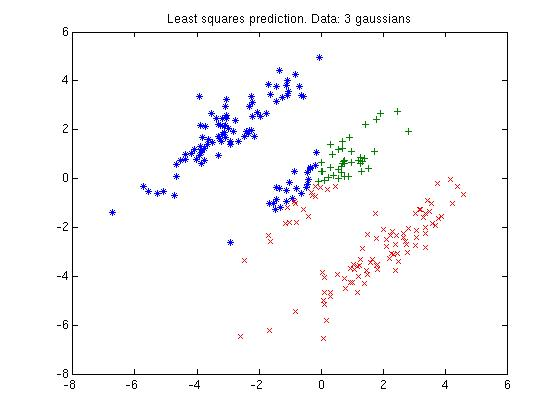
\includegraphics[scale=.75]{lsqPrediction.jpg}

I observe that, in the middle cluster, many points are misclassified as belonging to other classes. This could probably be due to the sensitivity of least squares to outliers.

\subsection{b}
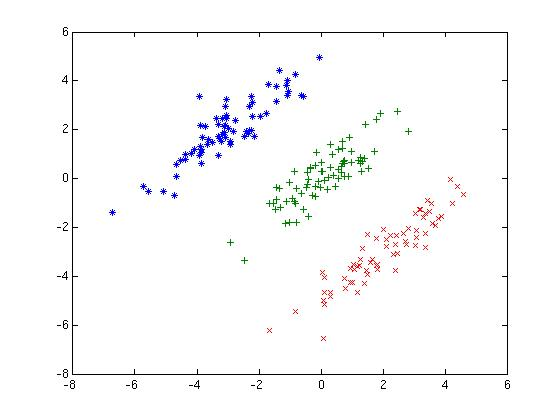
\includegraphics[scale=.75]{logisticPrediction.jpg}

I observe that, using least squares regression, classification is almost perfect!

\subsection{Code}
\verbatiminput{logistic.m}

\section{4}
\subsection{a}
Let $\sum_{i=3}^{N}y_{i}\ga_{i} = k$. Then, from condition 1, $y_{1}\ga_{1} +  y_{2}\ga_{2} = -k$. The same condition should hold when $(\ga_{1}, \ga_{2})$ are modified to $(\bar{\ga}_{1}, \bar{\ga}_{2})$. So, we have $y_{1}\bar{\ga}_{1} +  y_{2}\bar{\ga}_{2} = -k$.

So, $y_{1}\ga_{1} +  y_{2}\ga_{2} = y_{1}\bar{\ga}_{1} +  y_{2}\bar{\ga}_{2} = -k$.

When $y_{1} = y_{2}$, multiplying both sides by $y_{1}$, we get: $\ga_{1} + \ga_{2} = \bar{\ga}_{1} + \bar{\ga}_{2}$. From condition 2, all these are non-negative. So, $\bar{\ga}_{2} = \ga_{1} + \ga_{2} - \bar{\ga}_{1} \geq \ga_{1} + \ga_{2}$.

When $y_{1} \neq y_{2}$, as $y_{1}y_{2} = -1$, multiplying both sides by $y_{2}$, we get: $\ga_{2} - \ga_{1} = -\bar{\ga}_{1} + \bar{\ga}_{2}$. From condition 2, all these are non-negative. So, $\hat{\ga}_{2} \geq \ga_{2} - \ga_{1}$.

\subsection{b}
As noted earlier, $y_{1}\ga_{1} +  y_{2}\ga_{2} = y_{1}\bar{\ga}_{1} +  y_{2}\bar{\ga}_{2} = -k$. Using $s = y_{1}y_{2}$, by multiplication by $y_{1}$: $\ga_{1} +  y_{1}y_{2}\ga_{2} = -y_{1}k$, which yields $\ga_{1} +  s\ga_{2} = -y_{1}k = \gamma$.

Let $v_{i} = \sum_{j=3}^{N}y_{j}\ga_{j}K_{i,j}$ for i = 1 or 2.

Using the above identities, we get:
\begin{eqnarray*}
\sum_{i=1}^{N} \ga_{i} &=& \gamma - s\ga_{2} + \ga_{2} + k'' \\
\sum_{i}\sum_{j} y_{i}y_{j} \ga_{i} \ga_{j}K_{i,j} &=& K_{1,1}(\gamma - s\ga)^{2} + K_{2,2}\ga_{2}^{2} + \\
&& 2sK_{1,2}(\gamma - s\ga_{2})\ga_{2} + 2v_{1}y_{1}(\gamma - s\ga_{2}) + 2y_{2}\ga_{2}v_{2} + k'\\
\end{eqnarray*}
Above, $k' = \sum_{i=3}^{N}\sum_{i=3}^{N}y_{i}y_{j} \ga_{i} \ga_{j}K_{i,j}$ and $k''$ are constants wrt $\ga_{2}$, but can depend on other $\ga_i$.

\begin{eqnarray*}
\therefore w(\ga_2) &=& \sum_{i} \ga_{i} - \frac{1}{2}\sum_{i}\sum_{j} y_{i}y_{j} \ga_{i} \ga_{j}K_{i,j}\\
&=& \gamma - s\ga_{2} + \ga_{2}  + k'' -2^{-1}[ K_{1,1}(\gamma - s\ga)^{2} + K_{2,2}\ga_{2}^{2} + \\
&& 2sK_{1,2}(\gamma - s\ga_{2})\ga_{2} + 2v_{1}y_{1}(\gamma - s\ga_{2}) + 2y_{2}\ga_{2}v_{2} + k']\\
\end{eqnarray*}


\subsection{c}
$\frac{w(\ga_{2})}{d\ga_{2}} = -s + 1 + sK_{1,1}(\gamma - s\ga_{2}) - K_{2,2}\ga_{2} - sK_{1,2}(\gamma - 2s\ga_{2}) + y_{1}sv_{1}2^{-1} - y_{2}v_{2}2^{-1}$.

Setting this to 0, and using $s^{2} = 1, y_{1}s = y_{2}$ and $d_{1,2} = K_{1,1} + K_{2,2} - 2K_{1,2}$, we get: $d_{1,2}\bar{\ga}_2 =  -s + 1 + sK_{1,1}\gamma - sK_{1,2}\gamma +2^{-1}y_{2}v_{1} - 2^{-1}y_{2}v_{2}$.

We confirm that this is the maximum by the following: $\frac{d^{2}w(\ga_{2})}{d\ga_{2}^{2}} = -K_{1,1} - K_{2,2} + 2K_{1,2} = -\norm{x_{1} - x_{2}}^{2}\leq 0$.

\subsection{d}
Take $E_{i} = \sum_{j} \ga_{j}y_{j}K_{i,j} + w_{0} - y_{i}$ for i = 1 or 2.

\begin{eqnarray}
E_{1} - E_{2} &=& y_{2} - y_{1} + \sum_j \ga_{j}y_{j}K_{1,j} - \sum_j \ga_{j}y_{j}K_{2,j} \\
&=& y_{2} - y_{1} + \ga_{1}y_{1}K_{1,1} + \ga_{2}y_{2}K_{1,2} + v_{1} \\
&& - \ga_{1}y_{1}K_{2,1} - \ga_{2}y_{2}K_{2,2} - v_{2}\\
&=& y_{2} - y_{1} + \gamma y_{1}K_{1,1} + v_{1} - v_{2} - \gamma y_{1}K_{2,1} - y_{2}\ga_{2}K_{1,1} \\
&& + \ga_{2}y_{2}K_{1,2} + y_{2}\ga_{2}K_{2,1} - \ga_{2}y_{2}K_{2,2}\\
\end{eqnarray}
Above, we have used the definitions of $\gamma$ and $v_{1}, v_{2}$ seen in part c, and the fact that $sy_{1} = y_{2}$.

So, $y_{2}(E_{1} - E_{2}) = 1-s + sK_{1,1}\gamma + y_{2}v_{1} - y_{2}v_{2} - s\gamma K_{1,2} - \ga_{2}(K_{1,1} - 2K_{1,2}+ K_{2,2})$.

Thus, comparing this with the equation for $\bar{\ga}$ derived in part c, we get: $\bar{\ga}_{2} = \ga_{2} + \frac{y_{2}(E_{1} - E_{2})}{d_{1,2}}$.

\subsubsection{Taking care of the constraints from part a}
The expression for $\bar{\ga}_{2}$ above gives the best step length for maximizing $W(\ga_{2})$ if we don't care about the constraints mentioned in part a. Also note that $W(\ga_{2})$ is a concave function, as we saw in part c. So, if the constraints do not allow us to select the maximal $\bar{\ga_{2}}$, we should select $\bar{\ga}_2$ to be a value within the feasible region, which is closest to the maximal $\bar{\ga}_2$. Below, we use this fact when incorporating the constraints from part a.

When $y_{1} = y_{2}$: $\bar{\ga}_{2} \geq \ga_{1} + \ga_{2}$. So, to satisfy this constraint, we pick: $\bar{\ga}_{2} = \min(\bar{\ga}_2, \ga_{1} + \ga_{2})$.

When $y_{1} \neq y_{2}$: $\hat{\ga}_{2} \geq \ga_{2} - \ga_{1}$. So, $\bar{\ga}_{2} = \max(\bar{\ga}_2, \ga_{2} - \ga_{1})$.

\subsubsection{Also satisfying the nonnegativity constraint}
We also want to impose the constraint: $\bar{\ga} \geq 0$ to the values of $\bar{\ga}_{2}$ specified above. Using the same reasoning, we want to pick a value within the feasible region (where all constraints are satisfied), which is closest to the maximal $\bar{\ga}_{2}$ we derived earlier.

So, when $y_{1} = y_{2}$: $\bar{\ga}_2 = \max(0, \min(\bar{\ga}_2, \ga_{1} + \ga_{2}))$

So, when $y_{1} \neq y_{2}$: $\bar{\ga}_2 = \max(0, \bar{\ga}_2, \ga_{2} - \ga_{1})$

\subsubsection{Finding \htext{$\bar{\ga}_{1}$}{..}}
We saw earlier that $y_{1}\ga_{1} +  y_{2}\ga_{2} = y_{1}\bar{\ga}_{1} +  y_{2}\bar{\ga}_{2}$. Multiplying both sides by $y_{1}$ and solving for $\bar{\ga}_{1}$, we get: $\bar{\ga}_{1} = \ga_{1} + y_{1}y_{2}(\ga_{2} - \bar{\ga}_2)$.

% \bibliographystyle{plain}
% \bibliography{../linAlg}


\end{document}
